% Options for packages loaded elsewhere
\PassOptionsToPackage{unicode}{hyperref}
\PassOptionsToPackage{hyphens}{url}
%
\documentclass[
]{article}
\usepackage{amsmath,amssymb}
\usepackage{iftex}
\ifPDFTeX
  \usepackage[T1]{fontenc}
  \usepackage[utf8]{inputenc}
  \usepackage{textcomp} % provide euro and other symbols
\else % if luatex or xetex
  \usepackage{unicode-math} % this also loads fontspec
  \defaultfontfeatures{Scale=MatchLowercase}
  \defaultfontfeatures[\rmfamily]{Ligatures=TeX,Scale=1}
\fi
\usepackage{lmodern}
\ifPDFTeX\else
  % xetex/luatex font selection
\fi
% Use upquote if available, for straight quotes in verbatim environments
\IfFileExists{upquote.sty}{\usepackage{upquote}}{}
\IfFileExists{microtype.sty}{% use microtype if available
  \usepackage[]{microtype}
  \UseMicrotypeSet[protrusion]{basicmath} % disable protrusion for tt fonts
}{}
\makeatletter
\@ifundefined{KOMAClassName}{% if non-KOMA class
  \IfFileExists{parskip.sty}{%
    \usepackage{parskip}
  }{% else
    \setlength{\parindent}{0pt}
    \setlength{\parskip}{6pt plus 2pt minus 1pt}}
}{% if KOMA class
  \KOMAoptions{parskip=half}}
\makeatother
\usepackage{xcolor}
\usepackage[margin=1in]{geometry}
\usepackage{color}
\usepackage{fancyvrb}
\newcommand{\VerbBar}{|}
\newcommand{\VERB}{\Verb[commandchars=\\\{\}]}
\DefineVerbatimEnvironment{Highlighting}{Verbatim}{commandchars=\\\{\}}
% Add ',fontsize=\small' for more characters per line
\usepackage{framed}
\definecolor{shadecolor}{RGB}{248,248,248}
\newenvironment{Shaded}{\begin{snugshade}}{\end{snugshade}}
\newcommand{\AlertTok}[1]{\textcolor[rgb]{0.94,0.16,0.16}{#1}}
\newcommand{\AnnotationTok}[1]{\textcolor[rgb]{0.56,0.35,0.01}{\textbf{\textit{#1}}}}
\newcommand{\AttributeTok}[1]{\textcolor[rgb]{0.13,0.29,0.53}{#1}}
\newcommand{\BaseNTok}[1]{\textcolor[rgb]{0.00,0.00,0.81}{#1}}
\newcommand{\BuiltInTok}[1]{#1}
\newcommand{\CharTok}[1]{\textcolor[rgb]{0.31,0.60,0.02}{#1}}
\newcommand{\CommentTok}[1]{\textcolor[rgb]{0.56,0.35,0.01}{\textit{#1}}}
\newcommand{\CommentVarTok}[1]{\textcolor[rgb]{0.56,0.35,0.01}{\textbf{\textit{#1}}}}
\newcommand{\ConstantTok}[1]{\textcolor[rgb]{0.56,0.35,0.01}{#1}}
\newcommand{\ControlFlowTok}[1]{\textcolor[rgb]{0.13,0.29,0.53}{\textbf{#1}}}
\newcommand{\DataTypeTok}[1]{\textcolor[rgb]{0.13,0.29,0.53}{#1}}
\newcommand{\DecValTok}[1]{\textcolor[rgb]{0.00,0.00,0.81}{#1}}
\newcommand{\DocumentationTok}[1]{\textcolor[rgb]{0.56,0.35,0.01}{\textbf{\textit{#1}}}}
\newcommand{\ErrorTok}[1]{\textcolor[rgb]{0.64,0.00,0.00}{\textbf{#1}}}
\newcommand{\ExtensionTok}[1]{#1}
\newcommand{\FloatTok}[1]{\textcolor[rgb]{0.00,0.00,0.81}{#1}}
\newcommand{\FunctionTok}[1]{\textcolor[rgb]{0.13,0.29,0.53}{\textbf{#1}}}
\newcommand{\ImportTok}[1]{#1}
\newcommand{\InformationTok}[1]{\textcolor[rgb]{0.56,0.35,0.01}{\textbf{\textit{#1}}}}
\newcommand{\KeywordTok}[1]{\textcolor[rgb]{0.13,0.29,0.53}{\textbf{#1}}}
\newcommand{\NormalTok}[1]{#1}
\newcommand{\OperatorTok}[1]{\textcolor[rgb]{0.81,0.36,0.00}{\textbf{#1}}}
\newcommand{\OtherTok}[1]{\textcolor[rgb]{0.56,0.35,0.01}{#1}}
\newcommand{\PreprocessorTok}[1]{\textcolor[rgb]{0.56,0.35,0.01}{\textit{#1}}}
\newcommand{\RegionMarkerTok}[1]{#1}
\newcommand{\SpecialCharTok}[1]{\textcolor[rgb]{0.81,0.36,0.00}{\textbf{#1}}}
\newcommand{\SpecialStringTok}[1]{\textcolor[rgb]{0.31,0.60,0.02}{#1}}
\newcommand{\StringTok}[1]{\textcolor[rgb]{0.31,0.60,0.02}{#1}}
\newcommand{\VariableTok}[1]{\textcolor[rgb]{0.00,0.00,0.00}{#1}}
\newcommand{\VerbatimStringTok}[1]{\textcolor[rgb]{0.31,0.60,0.02}{#1}}
\newcommand{\WarningTok}[1]{\textcolor[rgb]{0.56,0.35,0.01}{\textbf{\textit{#1}}}}
\usepackage{graphicx}
\makeatletter
\def\maxwidth{\ifdim\Gin@nat@width>\linewidth\linewidth\else\Gin@nat@width\fi}
\def\maxheight{\ifdim\Gin@nat@height>\textheight\textheight\else\Gin@nat@height\fi}
\makeatother
% Scale images if necessary, so that they will not overflow the page
% margins by default, and it is still possible to overwrite the defaults
% using explicit options in \includegraphics[width, height, ...]{}
\setkeys{Gin}{width=\maxwidth,height=\maxheight,keepaspectratio}
% Set default figure placement to htbp
\makeatletter
\def\fps@figure{htbp}
\makeatother
\setlength{\emergencystretch}{3em} % prevent overfull lines
\providecommand{\tightlist}{%
  \setlength{\itemsep}{0pt}\setlength{\parskip}{0pt}}
\setcounter{secnumdepth}{-\maxdimen} % remove section numbering
\ifLuaTeX
  \usepackage{selnolig}  % disable illegal ligatures
\fi
\usepackage{bookmark}
\IfFileExists{xurl.sty}{\usepackage{xurl}}{} % add URL line breaks if available
\urlstyle{same}
\hypersetup{
  pdftitle={More conditional relationships},
  pdfauthor={Prof.~Weldzius},
  hidelinks,
  pdfcreator={LaTeX via pandoc}}

\title{More conditional relationships}
\usepackage{etoolbox}
\makeatletter
\providecommand{\subtitle}[1]{% add subtitle to \maketitle
  \apptocmd{\@title}{\par {\large #1 \par}}{}{}
}
\makeatother
\subtitle{Homework 7}
\author{Prof.~Weldzius}
\date{Due Date: 2024-09-19}

\begin{document}
\maketitle

\section{A new question}\label{a-new-question}

Suppose we were concerned with whether some polls might give different
answers because of variation in who the poll is able to reach using that
method. People who take polls via landline phones (do you even know what
that is?) might differ from those who take surveys online. Or people
contacted using randomly generated phone numbers (RDD) may differ from
those contacted from a voter registration list that has had telephone
numbers merged onto it.

Polls were done using lots of different methods in 2020.

\section{Loading the data}\label{loading-the-data}

\begin{Shaded}
\begin{Highlighting}[]
\FunctionTok{require}\NormalTok{(tidyverse)}
\NormalTok{Pres2020.PV }\OtherTok{\textless{}{-}} \FunctionTok{read\_rds}\NormalTok{(}\AttributeTok{file=}\StringTok{"https://github.com/rweldzius/PSC4175\_F2024/raw/main/Data/Pres2020\_PV.Rds"}\NormalTok{)}
\NormalTok{Pres2020.PV }\OtherTok{\textless{}{-}}\NormalTok{ Pres2020.PV }\SpecialCharTok{\%\textgreater{}\%}
                \FunctionTok{mutate}\NormalTok{(}\AttributeTok{Trump =}\NormalTok{ Trump}\SpecialCharTok{/}\DecValTok{100}\NormalTok{,}
                      \AttributeTok{Biden =}\NormalTok{ Biden}\SpecialCharTok{/}\DecValTok{100}\NormalTok{,}
                      \AttributeTok{margin =}\NormalTok{ Biden }\SpecialCharTok{{-}}\NormalTok{ Trump)}
\end{Highlighting}
\end{Shaded}

\begin{Shaded}
\begin{Highlighting}[]
\NormalTok{Pres2020.PV }\SpecialCharTok{\%\textgreater{}\%}
  \FunctionTok{count}\NormalTok{(Mode)}
\end{Highlighting}
\end{Shaded}

\begin{verbatim}
## # A tibble: 9 x 2
##   Mode                 n
##   <chr>            <int>
## 1 IVR                  1
## 2 IVR/Online          47
## 3 Live phone - RBS    13
## 4 Live phone - RDD    51
## 5 Online             366
## 6 Online/Text          1
## 7 Phone - unknown      1
## 8 Phone/Online        19
## 9 <NA>                29
\end{verbatim}

This raises the question of -- how do we visualization variation in a
variable by another variable? More specifically, how can we visualize
how the \texttt{margin} we get using one type of survey compares to the
\texttt{margin} from another type of poll? (We cannot use a scatterplot
because the data is from different observations (here polls).)

We could do this using earlier methods by \texttt{select}ing polls with
a specific interview method (``mode'') and then plotting the
\texttt{margin} (or \texttt{Trump} or \texttt{Biden}), but that will
produce a bunch of separate plots that may be hard to directly compare.
(In addition to having more things to look at we would want to make sure
that the scale of the x-axis and y-axis are similar.)

We can plot another ``layer'' of data in `\texttt{ggplot} using the
\texttt{fill} paramter. Previously we used it to make the graphs look
nice by choosing a particular color. But if we set \texttt{fill} to be a
variable in our \texttt{tibble} then \texttt{ggplot} will plot the data
seperately for each unique value in the named variable. So if we want to
plot the histogram of \texttt{margin} for two types of polls we can use
the \texttt{fill} argument in \texttt{ggplot} to tell R to produce
different fills depending on the value of that variable.

\begin{Shaded}
\begin{Highlighting}[]
\NormalTok{Pres2020.PV }\SpecialCharTok{\%\textgreater{}\%} 
  \FunctionTok{filter}\NormalTok{(Mode }\SpecialCharTok{==} \StringTok{"IVR/Online"} \SpecialCharTok{|}\NormalTok{ Mode }\SpecialCharTok{==} \StringTok{"Live phone {-} RDD"}\NormalTok{) }\SpecialCharTok{\%\textgreater{}\%}
    \FunctionTok{ggplot}\NormalTok{(}\FunctionTok{aes}\NormalTok{(}\AttributeTok{x=}\NormalTok{ margin, }\AttributeTok{fill =}\NormalTok{ Mode)) }\SpecialCharTok{+}     
  \FunctionTok{labs}\NormalTok{(}\AttributeTok{y =} \StringTok{"Number of Polls"}\NormalTok{,}
         \AttributeTok{x =} \StringTok{"Biden{-} Trump Margin"}\NormalTok{,}
         \AttributeTok{title =} \StringTok{"Biden{-}Trump Margin for Two Types of Polls"}\NormalTok{,}
        \AttributeTok{fill =} \StringTok{"Mode of Interview"}\NormalTok{) }\SpecialCharTok{+}
    \FunctionTok{geom\_histogram}\NormalTok{(}\AttributeTok{bins=}\DecValTok{10}\NormalTok{, }\AttributeTok{color=}\StringTok{"black"}\NormalTok{, }\AttributeTok{position=}\StringTok{"dodge"}\NormalTok{) }\SpecialCharTok{+} 
    \FunctionTok{scale\_x\_continuous}\NormalTok{(}\AttributeTok{breaks=}\FunctionTok{seq}\NormalTok{(}\SpecialCharTok{{-}}\NormalTok{.}\DecValTok{1}\NormalTok{,.}\DecValTok{2}\NormalTok{,}\AttributeTok{by=}\NormalTok{.}\DecValTok{05}\NormalTok{),}
                     \AttributeTok{labels=}\NormalTok{ scales}\SpecialCharTok{::}\FunctionTok{percent\_format}\NormalTok{(}\AttributeTok{accuracy =} \DecValTok{1}\NormalTok{))}
\end{Highlighting}
\end{Shaded}

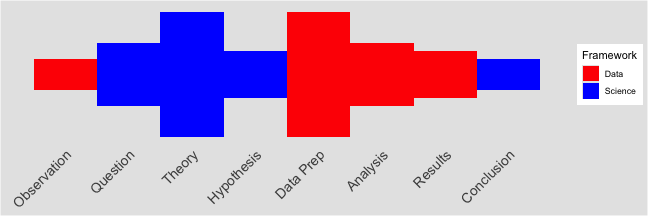
\includegraphics{psc4175_hw_7_files/figure-latex/unnamed-chunk-3-1.pdf}

\emph{Quick Exercise} Try running the code without the \texttt{filter}.
What do you observe? How useful is this? Why or why not?

\begin{Shaded}
\begin{Highlighting}[]
\CommentTok{\# INSERT CODE}
\end{Highlighting}
\end{Shaded}

While informative, it can be hard to compare the distribution of more
than two categories using such methods. To compare the variation across
more types of surveys we need to use a different visualization that
summarizes the variation in the variable of interest a bit more. One
common visualization is the \texttt{boxplot} which reports the mean,
25th percentile (i.e., the value of the data if we sort the data from
lowest to highest and take the value of the observation that is 25\% of
the way through), the 75th percentile, the range of values, and notable
outliers.

Let's see what the \texttt{boxplot} of survey mode looks like after we
first drop surveys that were conducted using modes that were hardly used
(or missing).

\begin{Shaded}
\begin{Highlighting}[]
\NormalTok{Pres2020.PV }\SpecialCharTok{\%\textgreater{}\%} 
  \FunctionTok{filter}\NormalTok{(Mode }\SpecialCharTok{!=} \StringTok{"IVR"} \SpecialCharTok{\&}\NormalTok{ Mode }\SpecialCharTok{!=} \StringTok{"Online/Text"} \SpecialCharTok{\&}\NormalTok{ Mode }\SpecialCharTok{!=} \StringTok{"Phone {-} unknown"} \SpecialCharTok{\&}\NormalTok{ Mode }\SpecialCharTok{!=} \StringTok{"NA"}\NormalTok{) }\SpecialCharTok{\%\textgreater{}\%}
  \FunctionTok{ggplot}\NormalTok{(}\FunctionTok{aes}\NormalTok{(}\AttributeTok{x =}\NormalTok{ Mode, }\AttributeTok{y =}\NormalTok{ margin)) }\SpecialCharTok{+} 
    \FunctionTok{labs}\NormalTok{(}\AttributeTok{x =} \StringTok{"Mode of Survey Interview"}\NormalTok{,}
         \AttributeTok{y =} \StringTok{"Biden{-} Trump Margin"}\NormalTok{,}
         \AttributeTok{title =} \StringTok{"2020 Popular Vote Margin by Type of Poll"}\NormalTok{) }\SpecialCharTok{+}
    \FunctionTok{geom\_boxplot}\NormalTok{(}\AttributeTok{fill =} \StringTok{"slateblue"}\NormalTok{) }\SpecialCharTok{+}
    \FunctionTok{scale\_y\_continuous}\NormalTok{(}\AttributeTok{breaks=}\FunctionTok{seq}\NormalTok{(}\SpecialCharTok{{-}}\NormalTok{.}\DecValTok{1}\NormalTok{,.}\DecValTok{2}\NormalTok{,}\AttributeTok{by=}\NormalTok{.}\DecValTok{05}\NormalTok{),}
                     \AttributeTok{labels=}\NormalTok{ scales}\SpecialCharTok{::}\FunctionTok{percent\_format}\NormalTok{(}\AttributeTok{accuracy =} \DecValTok{1}\NormalTok{))}
\end{Highlighting}
\end{Shaded}

\includegraphics{psc4175_hw_7_files/figure-latex/unnamed-chunk-5-1.pdf}

We can also flip the graph if we think it makes more sense to display it
in a different orientation using \texttt{coord\_flip}. (We could, of
course, also redefine the x and y variables in the `\texttt{ggplot}
object, but it is useful to have a command to do this to help you
determine which orientiation is most useful).

\begin{Shaded}
\begin{Highlighting}[]
\NormalTok{Pres2020.PV }\SpecialCharTok{\%\textgreater{}\%} 
  \FunctionTok{filter}\NormalTok{(Mode }\SpecialCharTok{!=} \StringTok{"IVR"} \SpecialCharTok{\&}\NormalTok{ Mode }\SpecialCharTok{!=} \StringTok{"Online/Text"} \SpecialCharTok{\&}\NormalTok{ Mode }\SpecialCharTok{!=} \StringTok{"Phone {-} unknown"} \SpecialCharTok{\&}\NormalTok{ Mode }\SpecialCharTok{!=} \StringTok{"NA"}\NormalTok{) }\SpecialCharTok{\%\textgreater{}\%}
  \FunctionTok{ggplot}\NormalTok{(}\FunctionTok{aes}\NormalTok{(}\AttributeTok{x =}\NormalTok{ Mode, }\AttributeTok{y =}\NormalTok{ margin)) }\SpecialCharTok{+} 
    \FunctionTok{labs}\NormalTok{(}\AttributeTok{x =} \StringTok{"Mode of Survey Interview"}\NormalTok{,}
         \AttributeTok{y =} \StringTok{"Biden{-} Trump Margin"}\NormalTok{,}
         \AttributeTok{title =} \StringTok{"2020 Popular Vote Margin by Type of Poll"}\NormalTok{) }\SpecialCharTok{+}
    \FunctionTok{geom\_boxplot}\NormalTok{(}\AttributeTok{fill =} \StringTok{"slateblue"}\NormalTok{) }\SpecialCharTok{+}
    \FunctionTok{scale\_y\_continuous}\NormalTok{(}\AttributeTok{breaks=}\FunctionTok{seq}\NormalTok{(}\SpecialCharTok{{-}}\NormalTok{.}\DecValTok{1}\NormalTok{,.}\DecValTok{2}\NormalTok{,}\AttributeTok{by=}\NormalTok{.}\DecValTok{05}\NormalTok{),}
                     \AttributeTok{labels=}\NormalTok{ scales}\SpecialCharTok{::}\FunctionTok{percent\_format}\NormalTok{(}\AttributeTok{accuracy =} \DecValTok{1}\NormalTok{)) }\SpecialCharTok{+}
    \FunctionTok{coord\_flip}\NormalTok{()}
\end{Highlighting}
\end{Shaded}

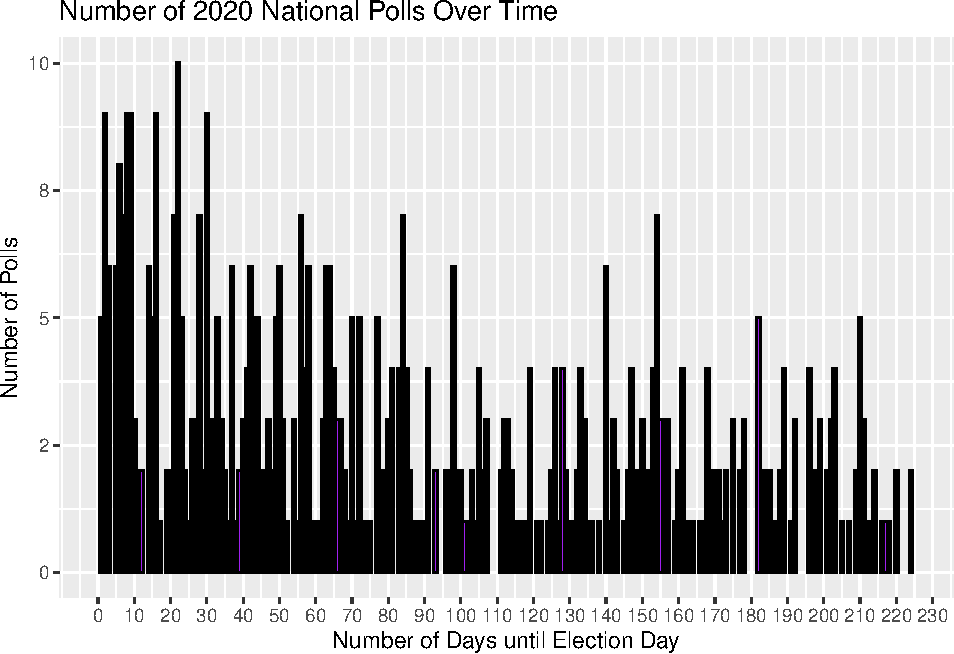
\includegraphics{psc4175_hw_7_files/figure-latex/unnamed-chunk-6-1.pdf}

A downside of the boxplot is that it can be hard to tell how the data
varies within each box. Is it equally spread out? How much data are
contained in the lines (which are simply 1.5 times the height of the
box)? To get a better handle on this we can use a ``violin'' plot that
dispenses with a standard box and instead tries to plot the distribution
of data within each category.

\begin{Shaded}
\begin{Highlighting}[]
\NormalTok{Pres2020.PV }\SpecialCharTok{\%\textgreater{}\%} 
  \FunctionTok{filter}\NormalTok{(Mode }\SpecialCharTok{!=} \StringTok{"IVR"} \SpecialCharTok{\&}\NormalTok{ Mode }\SpecialCharTok{!=} \StringTok{"Online/Text"} \SpecialCharTok{\&}\NormalTok{ Mode }\SpecialCharTok{!=} \StringTok{"Phone {-} unknown"} \SpecialCharTok{\&}\NormalTok{ Mode }\SpecialCharTok{!=} \StringTok{"NA"}\NormalTok{) }\SpecialCharTok{\%\textgreater{}\%}
  \FunctionTok{ggplot}\NormalTok{(}\FunctionTok{aes}\NormalTok{(}\AttributeTok{x=}\NormalTok{Mode, }\AttributeTok{y=}\NormalTok{margin)) }\SpecialCharTok{+} 
    \FunctionTok{xlab}\NormalTok{(}\StringTok{"Mode"}\NormalTok{) }\SpecialCharTok{+} 
    \FunctionTok{ylab}\NormalTok{(}\StringTok{"Biden{-} Trump Margin"}\NormalTok{) }\SpecialCharTok{+}
    \FunctionTok{geom\_violin}\NormalTok{(}\AttributeTok{fill=}\StringTok{"slateblue"}\NormalTok{)}
\end{Highlighting}
\end{Shaded}

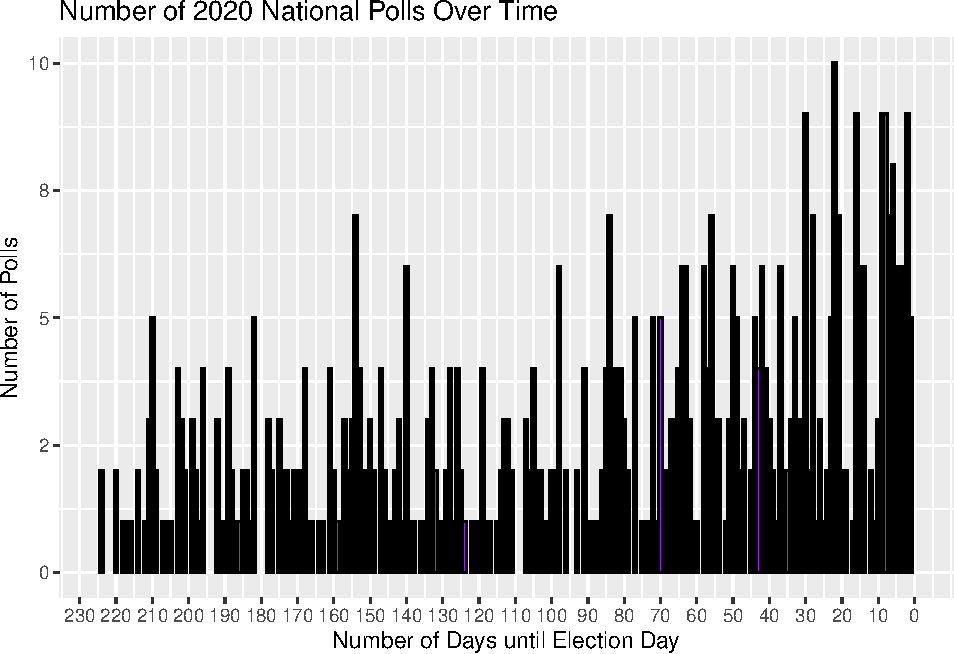
\includegraphics{psc4175_hw_7_files/figure-latex/unnamed-chunk-7-1.pdf}

It is also hard to know \textbf{how much} data is being plotted. If some
modes have 1000 polls and others have only 5 that seems relevant.

\emph{Quick Exercise} We have looked at the difference in
\texttt{margin}. How about differences in the percent who report
supporting \texttt{Biden} and \texttt{Trump}? What do you observe. Does
this suggest that the different ways of contacting respondents may
matter in terms of who responds? Is there something else that may
explain the differences (i.e., what are we assuming when making this
comparison)?

\begin{Shaded}
\begin{Highlighting}[]
\CommentTok{\# INSERT CODE HERE}
\end{Highlighting}
\end{Shaded}

\emph{Quick Exercise} Some claims have been made that polls that used
multiple ways of contacting respondents were better than polls that used
just one. Can you evaluate whether there were differences in so-called
``mixed-mode'' surveys compared to single-mode surveys? (This requires
you to define a new variable based on \texttt{Mode} indicating whether
survey is mixed-mode or not.)

\begin{Shaded}
\begin{Highlighting}[]
\CommentTok{\# INSERT CODE HERE}
\end{Highlighting}
\end{Shaded}

\section{Continuous Variable By Continuous Variable
(Scatterplot)}\label{continuous-variable-by-continuous-variable-scatterplot}

When we have two continuous variables we use a scatterplot to visualize
the relationship. A scatterplot is simply a graph of every point in
(x,y) where x is the value associated with the x-variable and y is the
value associated with the y-variable. For example, we may want to see
how support for Trump and Biden within a poll varies. So each
observation is a poll of the national popular vote and we are going to
plot the percentage of respondents in each poll supporting Biden against
the percentage who support Trump.

To include two variables we are going to change our aesthetic to define
both an x variable and a y variable -- here
\texttt{aes(x\ =\ Biden,\ y\ =\ Trump)} and we are going to label and
scale the axes appropriately.

\begin{Shaded}
\begin{Highlighting}[]
\NormalTok{Pres2020.PV }\SpecialCharTok{\%\textgreater{}\%}
  \FunctionTok{ggplot}\NormalTok{(}\FunctionTok{aes}\NormalTok{(}\AttributeTok{x =}\NormalTok{ Biden, }\AttributeTok{y =}\NormalTok{ Trump)) }\SpecialCharTok{+} 
  \FunctionTok{labs}\NormalTok{(}\AttributeTok{title=}\StringTok{"Biden and Trump Support in 2020 National Popular Vote"}\NormalTok{,}
       \AttributeTok{y =} \StringTok{"Trump Support"}\NormalTok{,}
       \AttributeTok{x =} \StringTok{"Biden Support"}\NormalTok{) }\SpecialCharTok{+} 
  \FunctionTok{geom\_point}\NormalTok{(}\AttributeTok{color=}\StringTok{"purple"}\NormalTok{) }\SpecialCharTok{+} 
    \FunctionTok{scale\_y\_continuous}\NormalTok{(}\AttributeTok{breaks=}\FunctionTok{seq}\NormalTok{(}\DecValTok{0}\NormalTok{,}\DecValTok{1}\NormalTok{,}\AttributeTok{by=}\NormalTok{.}\DecValTok{05}\NormalTok{),}
                     \AttributeTok{labels=}\NormalTok{ scales}\SpecialCharTok{::}\FunctionTok{percent\_format}\NormalTok{(}\AttributeTok{accuracy =} \DecValTok{1}\NormalTok{)) }\SpecialCharTok{+}
  \FunctionTok{scale\_x\_continuous}\NormalTok{(}\AttributeTok{breaks=}\FunctionTok{seq}\NormalTok{(}\DecValTok{0}\NormalTok{,}\DecValTok{1}\NormalTok{,}\AttributeTok{by=}\NormalTok{.}\DecValTok{05}\NormalTok{),}
                     \AttributeTok{labels=}\NormalTok{ scales}\SpecialCharTok{::}\FunctionTok{percent\_format}\NormalTok{(}\AttributeTok{accuracy =} \DecValTok{1}\NormalTok{))}
\end{Highlighting}
\end{Shaded}

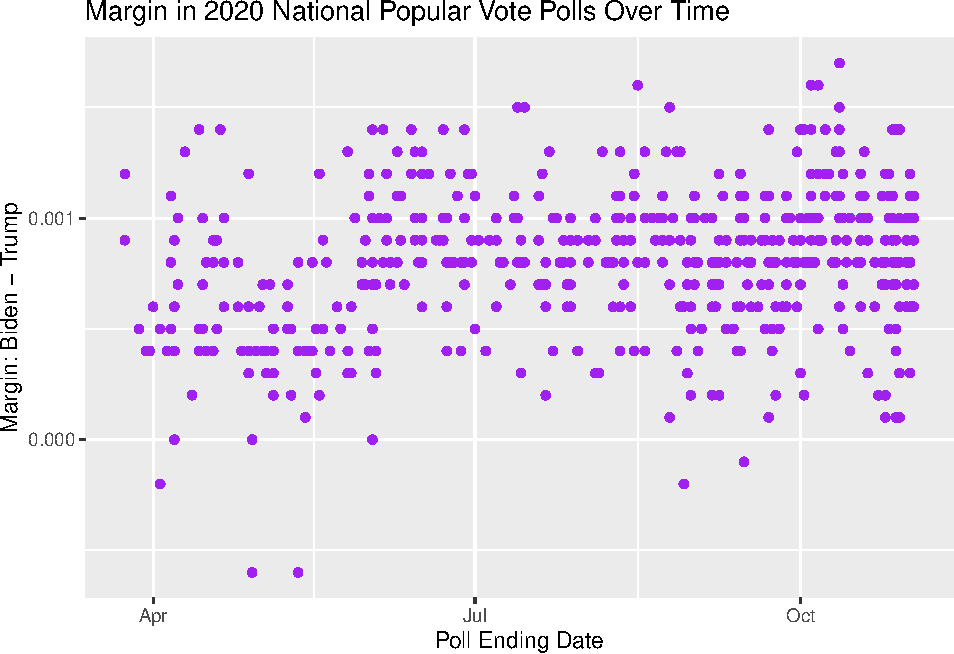
\includegraphics{psc4175_hw_7_files/figure-latex/unnamed-chunk-10-1.pdf}

The results are intriguing! First the data seems like it falls along a
grid. This is because of how poll results are reported in terms of
percentage points and it highlights that even continuous variables may
be reported in discrete values. This is consequential because it is hard
to know how many polls are associated with each point on the graph. How
many polls are at the point (Biden 50\%, Trump 45\%)? This matters for
trying to determine what the relationship might be. Second, it is clear
that there are some questions that need to be asked -- why doesn't
\texttt{Biden\ +\ Trump\ =\ 100\textbackslash{}\%}?

To try to display how many observations are located at each point we
have two tools at our disposal. First, we can alter the ``alpha
transparency'' by setting \texttt{alpha-.5} in the \texttt{geom\_point}
call. By setting a low level of transparency, this means that the point
will become less transparent as more points occur at the same
coordinate. Thus, a faint point indicates that only a single poll
(observation) is located at a coordinate whereas a solid point indicates
that there are many polls. When we apply this to the scatterplot you can
immediately see that most of the polls are located in the neighborhood
of Biden 50\%, Trump 42\%.

\begin{Shaded}
\begin{Highlighting}[]
\NormalTok{Pres2020.PV }\SpecialCharTok{\%\textgreater{}\%}
  \FunctionTok{ggplot}\NormalTok{(}\FunctionTok{aes}\NormalTok{(}\AttributeTok{x =}\NormalTok{ Biden, }\AttributeTok{y =}\NormalTok{ Trump)) }\SpecialCharTok{+} 
  \FunctionTok{labs}\NormalTok{(}\AttributeTok{title=}\StringTok{"Biden and Trump Support in 2020 National Popular Vote"}\NormalTok{,}
       \AttributeTok{y =} \StringTok{"Trump Support"}\NormalTok{,}
       \AttributeTok{x =} \StringTok{"Biden Support"}\NormalTok{) }\SpecialCharTok{+} 
  \FunctionTok{geom\_point}\NormalTok{(}\AttributeTok{color=}\StringTok{"purple"}\NormalTok{,}\AttributeTok{alpha =}\NormalTok{ .}\DecValTok{3}\NormalTok{) }\SpecialCharTok{+} 
    \FunctionTok{scale\_y\_continuous}\NormalTok{(}\AttributeTok{breaks=}\FunctionTok{seq}\NormalTok{(}\DecValTok{0}\NormalTok{,}\DecValTok{1}\NormalTok{,}\AttributeTok{by=}\NormalTok{.}\DecValTok{05}\NormalTok{),}
                     \AttributeTok{labels=}\NormalTok{ scales}\SpecialCharTok{::}\FunctionTok{percent\_format}\NormalTok{(}\AttributeTok{accuracy =} \DecValTok{1}\NormalTok{)) }\SpecialCharTok{+}
  \FunctionTok{scale\_x\_continuous}\NormalTok{(}\AttributeTok{breaks=}\FunctionTok{seq}\NormalTok{(}\DecValTok{0}\NormalTok{,}\DecValTok{1}\NormalTok{,}\AttributeTok{by=}\NormalTok{.}\DecValTok{05}\NormalTok{),}
                     \AttributeTok{labels=}\NormalTok{ scales}\SpecialCharTok{::}\FunctionTok{percent\_format}\NormalTok{(}\AttributeTok{accuracy =} \DecValTok{1}\NormalTok{))}
\end{Highlighting}
\end{Shaded}

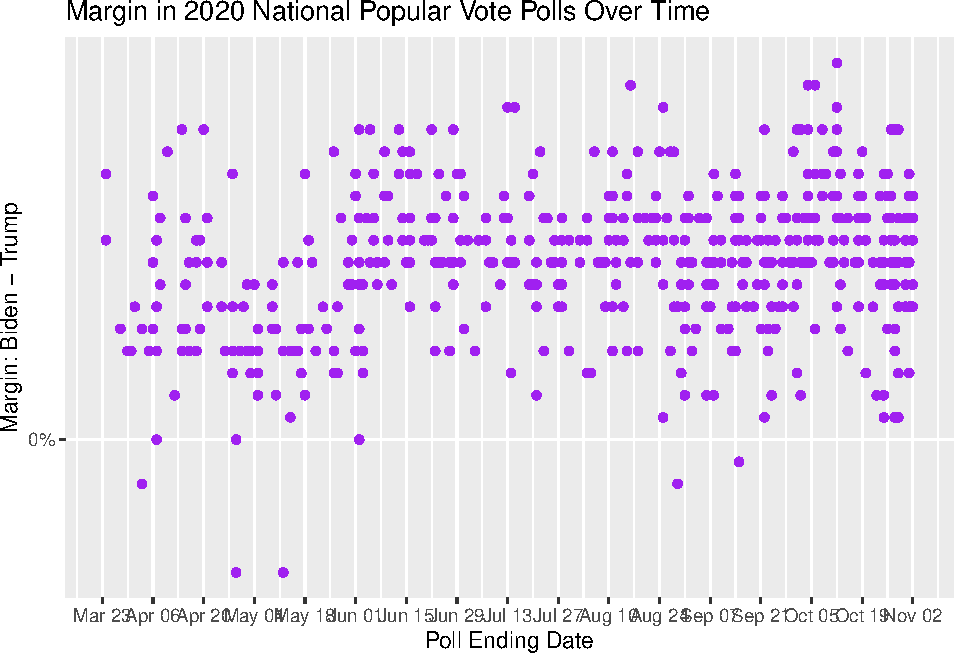
\includegraphics{psc4175_hw_7_files/figure-latex/unnamed-chunk-11-1.pdf}

However, the grid-like nature of the plot is still somewhat hard to
interpret as it can be hard to discern variations in color gradient.
Another tool is to add a tiny bit of randomness to the x and y values
associated with each plot. Instead of values being constrained to vary
by a full percentage point, for example, the jitter allows it to vary by
less. To do so we replace \texttt{geom\_point} with
\texttt{geom\_jitter}.

\begin{Shaded}
\begin{Highlighting}[]
\NormalTok{Pres2020.PV }\SpecialCharTok{\%\textgreater{}\%}
  \FunctionTok{ggplot}\NormalTok{(}\FunctionTok{aes}\NormalTok{(}\AttributeTok{x =}\NormalTok{ Biden, }\AttributeTok{y =}\NormalTok{ Trump)) }\SpecialCharTok{+} 
  \FunctionTok{labs}\NormalTok{(}\AttributeTok{title=}\StringTok{"Biden and Trump Support in 2020 National Popular Vote"}\NormalTok{,}
       \AttributeTok{y =} \StringTok{"Trump Support"}\NormalTok{,}
       \AttributeTok{x =} \StringTok{"Biden Support"}\NormalTok{) }\SpecialCharTok{+} 
  \FunctionTok{geom\_jitter}\NormalTok{(}\AttributeTok{color=}\StringTok{"purple"}\NormalTok{,}\AttributeTok{alpha =}\NormalTok{ .}\DecValTok{5}\NormalTok{) }\SpecialCharTok{+} 
    \FunctionTok{scale\_y\_continuous}\NormalTok{(}\AttributeTok{breaks=}\FunctionTok{seq}\NormalTok{(}\DecValTok{0}\NormalTok{,}\DecValTok{1}\NormalTok{,}\AttributeTok{by=}\NormalTok{.}\DecValTok{05}\NormalTok{),}
                     \AttributeTok{labels=}\NormalTok{ scales}\SpecialCharTok{::}\FunctionTok{percent\_format}\NormalTok{(}\AttributeTok{accuracy =} \DecValTok{1}\NormalTok{)) }\SpecialCharTok{+}
  \FunctionTok{scale\_x\_continuous}\NormalTok{(}\AttributeTok{breaks=}\FunctionTok{seq}\NormalTok{(}\DecValTok{0}\NormalTok{,}\DecValTok{1}\NormalTok{,}\AttributeTok{by=}\NormalTok{.}\DecValTok{05}\NormalTok{),}
                     \AttributeTok{labels=}\NormalTok{ scales}\SpecialCharTok{::}\FunctionTok{percent\_format}\NormalTok{(}\AttributeTok{accuracy =} \DecValTok{1}\NormalTok{)) }
\end{Highlighting}
\end{Shaded}

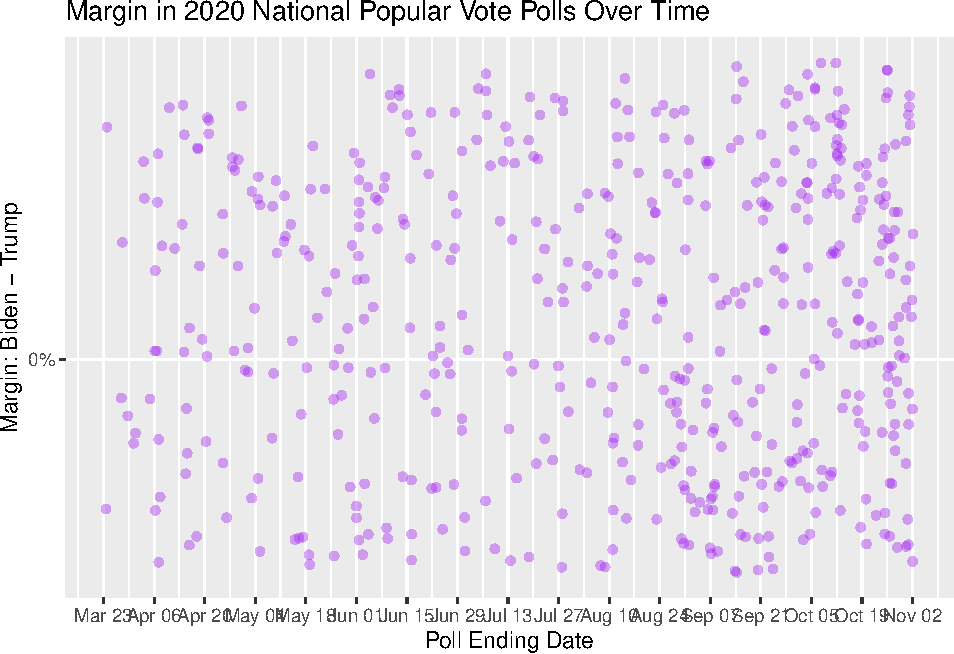
\includegraphics{psc4175_hw_7_files/figure-latex/unnamed-chunk-12-1.pdf}

Note how much the visualization changes. Whereas before the eye was
focused on -- and arguably distracted by -- the grid-like orientation
imposed by the measurement, once we jitter the points we are immediately
made aware of the relationship between the two variables. While we are
indeed slightly changing our data by adding random noise, the payoff is
that the visualization arguably better highlights the nature of the
relationship. Insofar the goal of visualization is communication, this
trade-off seems worthwhile in this instance. But here again is where
data science is sometimes art as much as science. The decision of which
visualization to use depends on what you think most effectively
communicates the nature of the relationship to the reader.

We can also look at the accuracy of a poll as a function of the sample
size. This is also a relationship between two continuous variables --
hence a scatterplot! Are polls with more respondents more accurate?
There is one poll with nearly 80,000 respondents that we will filter out
to me able to show a reasonable scale. Note that we are going to use
\texttt{labels\ =\ scales::comma} when plotting the x-axis to report
numbers with commas for readability.

\begin{Shaded}
\begin{Highlighting}[]
\NormalTok{Pres2020.PV }\SpecialCharTok{\%\textgreater{}\%}
  \FunctionTok{filter}\NormalTok{(SampleSize }\SpecialCharTok{\textless{}} \DecValTok{50000}\NormalTok{) }\SpecialCharTok{\%\textgreater{}\%}
  \FunctionTok{mutate}\NormalTok{(}\AttributeTok{TrumpError =}\NormalTok{ Trump }\SpecialCharTok{{-}}\NormalTok{ RepCertVote}\SpecialCharTok{/}\DecValTok{100}\NormalTok{,}
         \AttributeTok{BidenError =}\NormalTok{ Biden }\SpecialCharTok{{-}}\NormalTok{ DemCertVote}\SpecialCharTok{/}\DecValTok{100}\NormalTok{) }\SpecialCharTok{\%\textgreater{}\%}
  \FunctionTok{ggplot}\NormalTok{(}\FunctionTok{aes}\NormalTok{(}\AttributeTok{x =}\NormalTok{ SampleSize, }\AttributeTok{y =}\NormalTok{ TrumpError)) }\SpecialCharTok{+} 
  \FunctionTok{labs}\NormalTok{(}\AttributeTok{title=}\StringTok{"Trump Polling Error in 2020 National Popular Vote as a function of Sample Size"}\NormalTok{,}
       \AttributeTok{y =} \StringTok{"Error: Trump Poll {-} Trump Certified Vote"}\NormalTok{,}
       \AttributeTok{x =} \StringTok{"Sample Size in Poll"}\NormalTok{) }\SpecialCharTok{+} 
  \FunctionTok{geom\_jitter}\NormalTok{(}\AttributeTok{color=}\StringTok{"purple"}\NormalTok{,}\AttributeTok{alpha =}\NormalTok{ .}\DecValTok{5}\NormalTok{) }\SpecialCharTok{+}
  \FunctionTok{scale\_y\_continuous}\NormalTok{(}\AttributeTok{breaks=}\FunctionTok{seq}\NormalTok{(}\SpecialCharTok{{-}}\NormalTok{.}\DecValTok{2}\NormalTok{,}\DecValTok{1}\NormalTok{,}\AttributeTok{by=}\NormalTok{.}\DecValTok{05}\NormalTok{),}
                     \AttributeTok{labels=}\NormalTok{ scales}\SpecialCharTok{::}\FunctionTok{percent\_format}\NormalTok{(}\AttributeTok{accuracy =} \DecValTok{1}\NormalTok{)) }\SpecialCharTok{+}
  \FunctionTok{scale\_x\_continuous}\NormalTok{(}\AttributeTok{breaks=}\FunctionTok{seq}\NormalTok{(}\DecValTok{0}\NormalTok{,}\DecValTok{30000}\NormalTok{,}\AttributeTok{by=}\DecValTok{5000}\NormalTok{),}
                     \AttributeTok{labels=}\NormalTok{ scales}\SpecialCharTok{::}\NormalTok{comma) }
\end{Highlighting}
\end{Shaded}

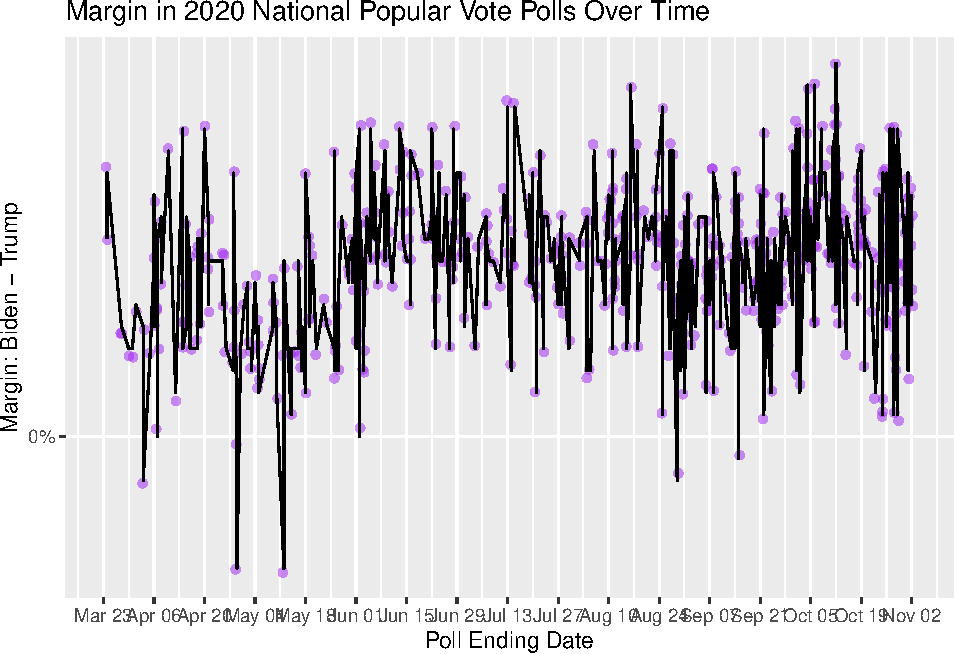
\includegraphics{psc4175_hw_7_files/figure-latex/unnamed-chunk-13-1.pdf}

In sum, we have tested Trump's theory that the MSM was biased against
him. We found that polls that underpredicted Trump \textbf{also}
underpredicted Biden. This is not what we would expect if the polls
favored one candidate over another.

\begin{Shaded}
\begin{Highlighting}[]
\NormalTok{Pres2020.PV }\SpecialCharTok{\%\textgreater{}\%}
  \FunctionTok{ggplot}\NormalTok{(}\FunctionTok{aes}\NormalTok{(}\AttributeTok{x =}\NormalTok{ Biden, }\AttributeTok{y =}\NormalTok{ Trump)) }\SpecialCharTok{+} 
  \FunctionTok{labs}\NormalTok{(}\AttributeTok{title=}\StringTok{"Biden and Trump Support in 2020 National Popular Vote"}\NormalTok{,}
       \AttributeTok{y =} \StringTok{"Trump Support"}\NormalTok{,}
       \AttributeTok{x =} \StringTok{"Biden Support"}\NormalTok{) }\SpecialCharTok{+} 
  \FunctionTok{geom\_jitter}\NormalTok{(}\AttributeTok{color=}\StringTok{"purple"}\NormalTok{,}\AttributeTok{alpha =}\NormalTok{ .}\DecValTok{5}\NormalTok{) }\SpecialCharTok{+} 
    \FunctionTok{scale\_y\_continuous}\NormalTok{(}\AttributeTok{breaks=}\FunctionTok{seq}\NormalTok{(}\DecValTok{0}\NormalTok{,}\DecValTok{1}\NormalTok{,}\AttributeTok{by=}\NormalTok{.}\DecValTok{05}\NormalTok{),}
                     \AttributeTok{labels=}\NormalTok{ scales}\SpecialCharTok{::}\FunctionTok{percent\_format}\NormalTok{(}\AttributeTok{accuracy =} \DecValTok{1}\NormalTok{)) }\SpecialCharTok{+}
  \FunctionTok{scale\_x\_continuous}\NormalTok{(}\AttributeTok{breaks=}\FunctionTok{seq}\NormalTok{(}\DecValTok{0}\NormalTok{,}\DecValTok{1}\NormalTok{,}\AttributeTok{by=}\NormalTok{.}\DecValTok{05}\NormalTok{),}
                     \AttributeTok{labels=}\NormalTok{ scales}\SpecialCharTok{::}\FunctionTok{percent\_format}\NormalTok{(}\AttributeTok{accuracy =} \DecValTok{1}\NormalTok{)) }
\end{Highlighting}
\end{Shaded}

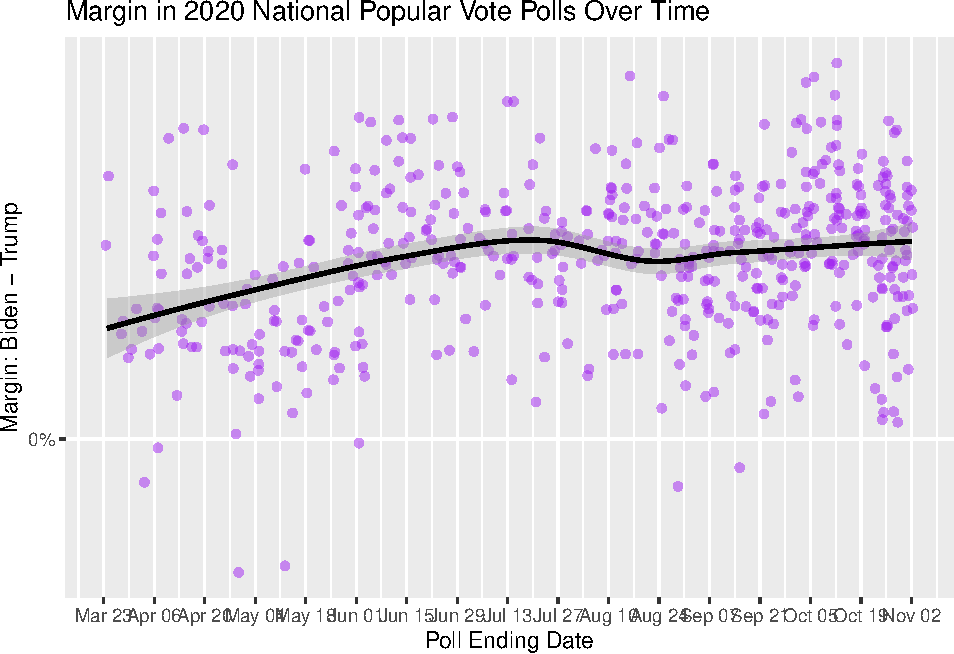
\includegraphics{psc4175_hw_7_files/figure-latex/unnamed-chunk-14-1.pdf}

What is an alternative explanation for these patterns? Why would polls
underpredict \emph{both} Trump and Biden?

Perhaps they were fielded earlier in the year, when more people were
interested in third party candidates, or hadn't made up their mind.
We'll turn to testing this theory next time!

\end{document}
